\chapter{Arbeitsaufgaben}
		\section{Protokoll Anfangskonsultation 18.04.2006}
		\subsection{Anwesende}
		\begin{itemize}
			\item Simon Wunderlich
			\item Andreas Tröger
			\item Frank Wilhelm
			\item Florian Scharl
			\item Sven Eckelmann
		\end{itemize}
		\subsection{Tagesordnung}
		\begin{itemize}
			\item Arten von Buchlisten
			\item Einteilung von Benutzern
			\item Sichtbarkeit von Kommentaren
			\item Funktionsweise der Suche
			\item Informationen für Bücher
			\item Verwendete Software im Softwaresystem
			\item Software für Graphen
			\item Nächste Sitzung
		\end{itemize}
			\subsection{Arten von Buchlisten}
			\begin{itemize}
				\item globale Bücherliste
				\item User können recherchieren und gefundene Bücher als BibTeX exportieren
				\item keine lokalen Listen für User
			\end{itemize}
			\subsection{Einteilung von Benutzern}
			\begin{itemize}
				\item Anonyme Nutzer (Gäste) können Suchen und Exportieren
				\item Registrierte Nutzer können zusätzlich Bücher hinzufügen/ändern/löschen/kommentieren
				\item Administratoren können zusätzlich Nutzer hinzufügen/ändern/löschen
			\end{itemize}
			\subsection{Sichtbarkeit von Kommentaren}
			\begin{itemize}
				\item registrierte Nutzer können Kommentare zu Buch verfassen
				\item jeder kann Kommentare zu Buch lesen
			\end{itemize}
			\subsection{Funktionsweise der Suche}
			\begin{itemize}
				\item Suche nach spezifischen Informationen (Titel, Autor, Verlag, ...)
				\item Freie Suche (Volltextsuche) nach Stichwörtern (auch in Bemerkungen, Stichworte, ...)
			\end{itemize}
			\subsection{Informationen für Bücher}
			\begin{itemize}
				\item Informationen laut Aufgabenbeschreibung:
					\begin{itemize}
						\item Art
						\item Titel
						\item Autor
						\item ISBN
						\item Jahr
						\item Ort
						\item Beschreibung
					\end{itemize}
				\item weitere Informationen laut DIN 1505 Teil 2
			\end{itemize}
			\subsection{Verwendete Software im Softwaresystem}
			\begin{itemize}
				\item DBS
					: MySQL 5.0
				\item Webserver
					: Apache 2.0
				\item Skriptsprache
					: PHP 5.1
			\end{itemize}
			\subsection{Software für Graphen}
			Vorschläge:
			\begin{itemize}
				\item xfig
				\item dot
				\item Microsoft Visio
			\end{itemize}
			\subsection{Nächste Sitzung}
			\begin{itemize}
				\item Treffen am 19.04. 15:15
				\item Besprechung einzelner Punkte des 1. Belegs
				\item Einteilen für Aufgaben
			\end{itemize}
		\begin{itemize}
			\item Protokolant: Sven Eckelmann
		\end{itemize}
\newpage
		\section{Sitzungsprotokoll 19.04.2006}
		\subsection{Anwesende}
		\begin{itemize}
			\item Simon Wunderlich
			\item Andreas Tröger
			\item Frank Wilhelm
			\item Florian Scharl
			\item Sven Eckelmann
		\end{itemize}
		\subsection{Tagesordnung}
		\begin{itemize}
			\item Aufteilung und Verteilung der Aufgaben zum 1. Teilbeleg
		\end{itemize}
			\subsection{Aufteilung und Verteilung der Aufgaben zum 1. Teilbeleg}
			Es wurden die zu bearbeitenden Aufgaben zur Erstellung des ersten Teilbeleges in folgende drei Komplexe aufgeteilt und an die jeweiligen Mitglieder des Teams verteilt:
			\begin{itemize}
				\item 1. Komplex - Sven Eckelmann, Frank Wilhelm
					\begin{itemize}	
						\item Kontextdiagramm
						\item Verhaltensmodells
						\item Prozessbeschreibung
						\item Planung in Form eines Gantt-Diagramms
					\end{itemize}
				\item 2. Komplex - Simon Wunderlich
					\begin{itemize}
						\item Definition der Nutzerschnittstellen
						\item Produktbeschreibung
						\item Entwicklungsumgebung
					\end{itemize}
				\item 3. Komplex - Andreas Tröger, Florian Scharl
					\begin{itemize}
						\item Datenkatalog
						\item Entity-Relationship-Modell
						\item Spezifikation wichtiger Qualifikationsanforderungen
					\end{itemize}
			\end{itemize}
			Chemnitz, 19.04.2006
			\begin{itemize}
				\item Protokolant: Florian Scharl
				\item Korrekturen: Sven Eckelmann
			\end{itemize}
\newpage
		\section{Sitzungsprotokoll 26.04.2006}
		\subsection{Anwesende}
		\begin{itemize}
			\item Simon Wunderlich
			\item Andreas Tröger
			\item Frank Wilhelm
			\item Florian Scharl
			\item Sven Eckelmann
		\end{itemize}
		\subsection{Tagesordnung}
		\begin{itemize}
			\item Aufteilung und Verteilung der Aufgaben zum 1. Teilbeleg
		\end{itemize}
			\subsection{Aufteilung und Verteilung der Aufgaben zum 1. Teilbeleg}
			\begin{itemize}
				\item Es wurden die Erbegnisse der einzelnen Aufgaben des erste Teilbeleg durchgesehen und Korrekturen besprochen.
				\item Weiteren Projektverlauf anhand des Gentt-Diagramms festgelegt.
				\item Aufgrund fehlenden Engagements und dem Versäumen aller bisherigen Treffen war es notwendig das Mitglied Benedikt Keil aus dem Projektteam zu entfernen. 
			\end{itemize}
			Chemnitz, 26.04.2006
			\begin{itemize}
				\item Protokolant: Andreas Tröger
				\item Korrekturen: Florian Scharl
			\end{itemize}
\newpage
		\section{Sitzungsprotokoll 03.05.2006}
		\subsection{Anwesende}
		\begin{itemize}
			\item Andreas Tröger
			\item Frank Wilhelm
			\item Florian Scharl
			\item Sven Eckelmann
		\end{itemize}
		\subsection{Tagesordnung}
		\begin{itemize}
			\item Korrekturen zum 1. Teilbeleg
		\end{itemize}
			\subsection{Korrekturen zum 1. Teilbeleg}
			\begin{itemize}
				\item Autoren Entität mit Relation zu Literatur hinzugefügt (ERD und Datenkatalog)
				\item Arten an Literatur im Datenkatalog definiert:
					\begin{itemize}
						\item Buch
						\item Artikel
						\item Broschüre
						\item Protokoll
						\item Anleitung
						\item Diplomarbeit
						\item Dissertation
						\item Techn. Bericht
						\item Unveröffentlicht
						\item Sonstiges
					\end{itemize}
				\item Suche auf Titel und Autoren
				\item Überarbeitung des Abschnitts 3.3 (Flexibilität)
			\end{itemize}
			Chemnitz, 03.05.2006
			\begin{itemize}
				\item Protokolant: Frank Wilhelm
			\end{itemize}
\newpage
		\section{Sitzungsprotokoll 10.05.2006}
		\subsection{Anwesende}
		\begin{itemize}
			\item Simon Wunderlich
			\item Andreas Tröger
			\item Frank Wilhelm
			\item Florian Scharl
			\item Sven Eckelmann
		\end{itemize}
		\subsection{Tagesordnung}
		\begin{itemize}
			\item Korrekturen zum 1. Teilbeleg
			\item Beleg2 Klassenaufteilung
		\end{itemize}
			\subsection{Korrekturen zum 1. Teilbeleg}
			\begin{itemize}
				\item Autoren bei Suchanfragen mit einbeziehen
			\end{itemize}
			\subsection{Beleg2 Klassenaufteilung}
			\begin{itemize}
					\item Eine Klassenaufteilung wurde festgelegt:
					\\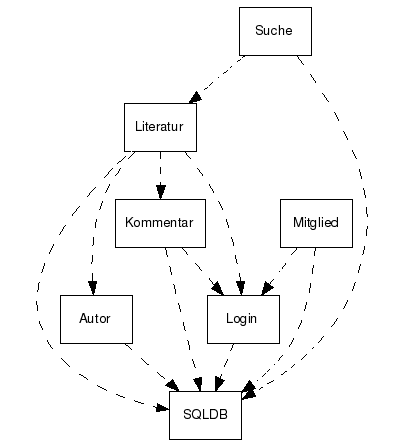
\includegraphics[scale=0.8]{../protokoll/2006_05_10.png}
					\item Generierung mit Doxygen soweit m"oglich
			\end{itemize}
			Chemnitz, 10.05.2006
			\begin{itemize}
				\item Protokolant: Simon Wunderlich
			\end{itemize}
\newpage
		\section{Protokoll 1. Pflichtkonsultation 30.05.2006}
		\subsection{Anwesende}
		\begin{itemize}
			\item Simon Wunderlich
			\item Andreas Tröger
			\item Frank Wilhelm
			\item Florian Scharl
			\item Sven Eckelmann
		\end{itemize}
		\subsection{Tagesordnung}
		\begin{itemize}
			\item Besprechung Teilbeleg 1
			\item Vorstellung Stand Teilbeleg 2
			\item Stand Projektarbeit
			\item Nächste Sitzung
		\end{itemize}
			\subsection{Besprechung Teilbeleg 1}
			\begin{itemize}
				\item fehlende Suchabfrage in Ereignistabelle und Datenkatalog
				\item kleine Fehler bei Formulierungen ({\it freier} Festplattenspeicher, Stil {\it der grafischen Oberfläche})
				\item keine Liste der Fehlercodes
			\end{itemize}
			\subsection{Vorstellung Stand Teilbeleg 2}
			\begin{itemize}
				\item Änderungsstand und Bearbeiter noch nicht aufgeführt
				\item Klassendiagramm nur ähnlich Moduldiagramm und kein UML-Klassendiagramm
			\end{itemize}
			\subsection{Stand Projektarbeit}
			\begin{itemize}
				\item Implementierung fast vollständig
				\item Systemtests am laufen bzw. in Vorbereitung
			\end{itemize}
			\subsection{Nächste Sitzung}
			\begin{itemize}
				\item Treffen am 7.6. 15:15
				\item Besprechung einzelner Punkte des 3. Belegs
			\end{itemize}
		\begin{itemize}
			\item Protokolant: Sven Eckelmann
		\end{itemize}
\newpage
		\section{Sitzungsprotokoll 07.06.2006}
		\subsection{Anwesende}
		\begin{itemize}
			\item Simon Wunderlich
			\item Andreas Tröger
			\item Frank Wilhelm
			\item Florian Scharl
			\item Sven Eckelmann
		\end{itemize}
		\subsection{Tagesordnung}
		\begin{itemize}
			\item Verteilung der Aufgaben zum 3. Teilbeleg
			\item Nächste Sitzung
			\item Nächste Pflichtkonsultation mit Betreuer
		\end{itemize}
			\subsection{Verteilung der Aufgaben zum 3. Teilbeleg}
			\begin{itemize}
			\item Programmdokumentation
			\begin{itemize}
			\item Definition der Interfaces in der Implementierungssprache -- Sven Eckelmann u. Frank 			Wilhelm
			\item Kommentierte Quelltexte -- Sven Eckelmann u. Frank Wilhelm
			\item Testplan -- Sven Eckelmann u. Frank Wilhelm
			\item Systemtest -- Sven Eckelmann u. Frank Wilhelm
			\item Abschlusseinschätzung -- Sven Eckelmann u. Frank Wilhelm
			\end{itemize}
			\item Systemhandbuch
			\begin{itemize}
			\item Installationsanleitung -- Simon Wunderlich
			\item Programm-Filesystem -- Andreas Tröger
			\item Administrationsanleitung -- Andreas Tröger
			\end{itemize}
			\item Anwenderdokumentation
			\begin{itemize}
			\item Produktzweck -- Florian Scharl
			\item Basismaschine und Ressourcenanforderungen -- Florian Scharl
			\item Nutzerklassen -- Florian Scharl
			\item Bedienungsanleitung -- Florian Scharl
			\item Helpsystem -- Florian Scharl
			\end{itemize}
			\item Übersicht über die Arbeitsaufgaben alle Teammitglieder während der gesamten Projektbearbeitung
			inkl. der Festlegungsprotokolle	-- Simon Wunderlich
			\end{itemize}
			Bemerkung: Die endgültige Festlegung erfolgt in der nächsten Sitzung nachdem jeder den Umfang 				seines Aufgabengebietes bzw. seiner Aufgabengebiete erschlossen hat.
			\subsection{Nächste Sitzung}
			\begin{itemize}
			\item Die nächste Sitzung findet am {\em 14.06.2006 um 15:15 Uhr im Raum 1/204 } statt.
			\end{itemize}
			\subsection{Nächste Pflichtkonsultation mit Betreuer}
			\begin{itemize}
			\item Die nächste Pflichtkonsultation mit Herrn Rentzsch findet am {\em 13.06.2006 um 13:10 Uhr im Raum 			1/B317 } statt.
			\end{itemize}
			Chemnitz, 07.06.2006
			\begin{itemize}
				\item Protokolant: Florian Scharl
			\end{itemize}
\newpage
		\section{Protokoll 2. Pflichtkonsultation 13.06.2006}
		\subsection{Anwesende}
		\begin{itemize}
			\item Simon Wunderlich
			\item Andreas Tröger
			\item Frank Wilhelm
			\item Florian Scharl
			\item Sven Eckelmann
		\end{itemize}
		\subsection{Tagesordnung}
		\begin{itemize}
			\item Besprechung Teilbeleg 2
			\item Vorstellung Stand Teilbeleg 3
			\item Nächste Sitzung
		\end{itemize}
			\subsection{Besprechung Teilbeleg 2}
			\begin{itemize}
				\item fehlende Trennung zwischen SQLDB-Klasse und Datenbank
				\item unklare Formulierung "Felder {\it mit Elementen} vom Typ..."
			\end{itemize}
			\subsection{Vorstellung Stand Teilbeleg 3}
			\begin{itemize}
				\item Implementierung weitgehend vollständig
				\item Tests werden fertiggestellt
				\item Anwender- und Systemdokumentation in Vorbereitung
			\end{itemize}
			\subsection{Nächste Sitzung}
			\begin{itemize}
				\item Treffen am 14.06. 15:15
				\item Besprechung einzelner Punkte des 3. Belegs
			\end{itemize}
		\begin{itemize}
			\item Protokolant: Sven Eckelmann
		\end{itemize}
\newpage
		\section{Sitzungsprotokoll 14.06.2006}
		\subsection{Anwesende}
		\begin{itemize}
			\item Simon Wunderlich
			\item Andreas Tröger
			\item Frank Wilhelm
			\item Florian Scharl
			\item Sven Eckelmann
		\end{itemize}
		\subsection{Tagesordnung}
		\begin{itemize}
			\item Besprechung Teilbeleg 3
		\end{itemize}
			\subsection{Besprechung Teilbeleg 3}
			\begin{itemize}
				\item Explizite Aufteilung noch zu erledigender Aufgaben
				\item Besprechung und Korrektur bisher vorhandener Teile
				\item Besprechung technischer Möglichkeiten zur Dokumentation der Oberfläche
				\item Archivierungsmöglichkeiten des Administrators (phpMyAdmin, mysqldump)
			\end{itemize}
		\begin{itemize}
			\item Protokolant: Sven Eckelmann
		\end{itemize}
\newpage
